\chapter{System Design and Implementation}
\section{Requirements and trust boundaries}

This chapter describes what was actually built, working outward from the trust boundary to the
controls that sit on each stage. The release is a local, single-user research prototype rather than a
service. It listens only on the machine that runs it and refuses any client or host header that is not
local (NFR-SEC-001, FR-UI-003). The bounded company-research route accepts a Companies House number on
its own, with no company name or website (FR-INT-001), but a named person must review and accept that
number before research can begin (FR-RES-001). One reviewed number is therefore the whole of what this
route needs to start. It fixes which registered company the work refers to, which is a narrower thing
than knowing that the company trades \citep{galanakis2026chrt,hardman2023small,nist2023airmf}.

Every item entering the system is labelled public, internal, restricted or synthetic, and each case keeps the purpose and the person behind it. The charter assigns the roles: the student operates the prototype, portfolio companies keep their confidentiality interests, and data owners or the university ethics body authorise any restricted or participant use. External-model processing is off by default and, when switched on, accepts only public or synthetic evidence (FR-EXT-005). The client sends \texttt{store=False} with every request, which controls what the provider saves as application state but not what it retains for abuse monitoring; Section~7.2 records the requests that were actually made under this route \citep{gebru2021datasheets,cddo2023genai,openai2026datacontrols}.

No output leaves the system without a person deciding that it may. Export of a report is blocked until the current version is approved (FR-REP-005), and reaching a company deck requires both a named review and a content-hash check (FR-RES-007). Four things sit outside the design entirely: remote or multi-user deployment, profiling of individuals, speculative valuation, and buy or sell recommendations. Direct live Companies House retrieval remains held at gate G2. The public-web route is built, and the external-model extraction provider was exercised in the bounded development smoke runs recorded in Section~7.2, but live public-web discovery, live capture and the frozen evaluation have not run. Table~\ref{tab:sys-requirements-trust-boundary}, in Appendix~\ref{app:requirements-traceability}, maps each control to the risk it addresses, chiefly misleading communication and untrusted content \citep{fca2024promotions,greshake2023indirect,nist2023airmf}.
\section{Architecture and local deployment}

The artefact runs as two local processes. Next.js renders the operator dashboard, and its server-side proxy calls a private FastAPI service, so the browser never reaches the API directly. Behind the API handlers, a single runtime object assembles the importing, source, workflow, reporting, intake and company-research services, and the command-line interface builds that same runtime, so both entry points exercise identical domain code rather than parallel implementations \citep{hevner2004design,peffers2007dsrm}.

SQLite holds the canonical identity, workflow, claim, review and audit records, with foreign keys enabled. Startup migrates the database to the declared head rather than creating tables directly, so the schema always has a stated version. Imported bytes and source captures are written once into local directories that Git ignores, verified by checksum and recorded by path, and approved exports are staged as manifest-backed bundles. Keeping relational metadata apart from the evidence bytes means a record can be traced to the exact file it came from \citep{pineau2021reproducibility,gebru2021datasheets}.

Docker Compose mirrors that two-process shape in pinned images. Only the dashboard is published to the local machine; it reaches the API over a private container network, both container file systems are read-only, and the API alone mounts the volume holding persistent state. Health, proxy, host, cross-site request forgery and migration checks exercise these mechanisms, and Figure~\ref{fig:sys-architecture-deployment-boundary} maps the resulting request and data path \citep{pineau2021reproducibility,nist2023airmf}.

Every control described here is a local one, sized to the attack surface of a single laptop rather than a hosted service; Section~7.5 states what a remote or multi-user release would additionally require \citep{nist2023airmf,cddo2023genai}.

\clearpage
\begin{figure}[p]
  \centering
  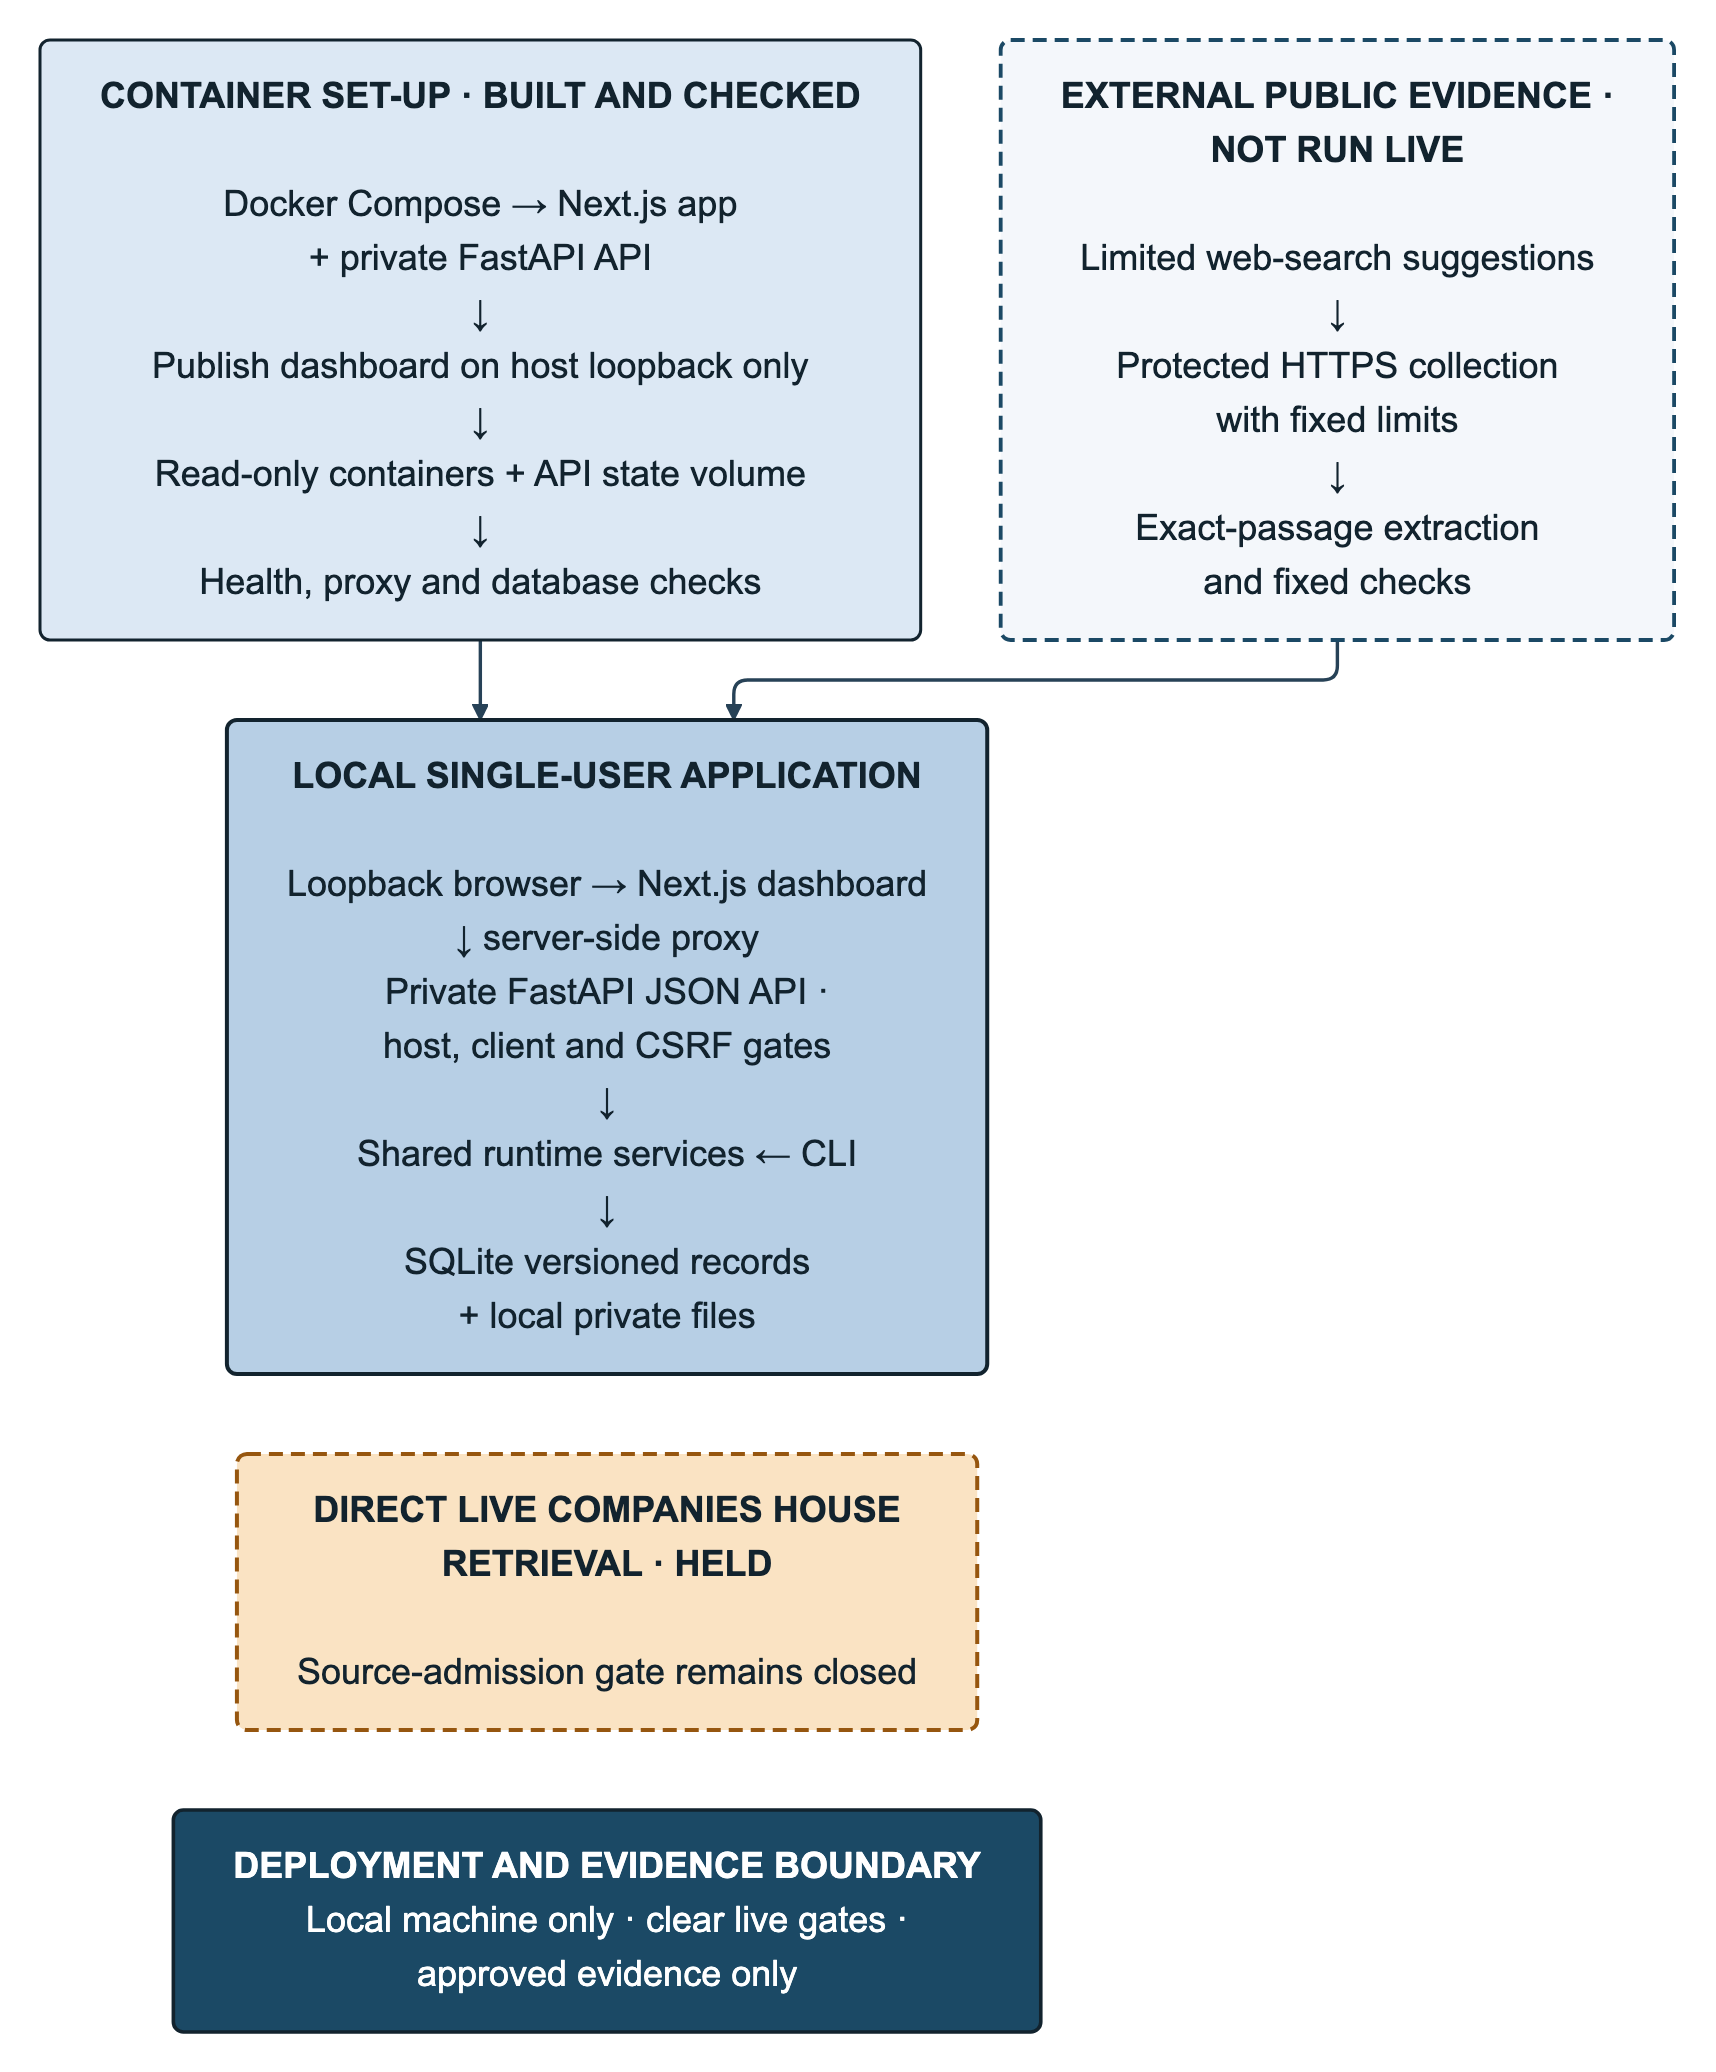
\includegraphics[width=\textwidth,height=0.82\textheight,keepaspectratio]{exhibits/sys_f1_architecture_deployment_boundary.png}
  \caption{Local architecture, deployment and external-boundary status. Author synthesis of the repository's contracts, its implementation and the local verification evidence.}
  \label{fig:sys-architecture-deployment-boundary}
\end{figure}
\clearpage
\section{Shared data definitions, storage and source records}

Shared meaning starts from a versioned catalogue. Each metric definition fixes a key, type, unit, sourceability, permitted aliases and one period meaning, and a hash over the catalogue stops a version being reused after its meaning has changed. Observations then bind a company, metric, period and raw submission together, and normalisation keeps the original value beside the cleaned one. Blank, explicit zero, none stated, not applicable, not reported, not found publicly, source unavailable and invalid are eight separate states, not interchangeable nulls. Distinguishing them is what allows a later reader to see why a figure is absent, though the eight categories are this project's definitions and would need a domain owner's agreement before wider use \citep{nikiforova2020quality,gebru2021datasheets}.

SQLite separates canonical companies and identifiers from submissions, observations, reporting periods, evidence, claims and reports. Foreign keys, uniqueness constraints and indexes protect relationships, while Alembic revisions 0001--0010 reproduce the ORM schema and incrementally add provenance, company-research and reviewed group-scope records. Revision 0010 was added after the dated evaluation snapshot, which Chapter~5 records at 0009; the results in that chapter therefore describe the earlier schema. Tests compare the migrated schema against the one the code expects, and exercise downgrade preflights. One weakness is visible here: many of the semantic states above are stored as strings or JSON and are enforced by application code rather than by the database, so the schema alone cannot guarantee they are used consistently \citep{pineau2021reproducibility,gebru2021datasheets}.

Imported files are hashed before persistence and published create-once under checksum-addressed paths. Connector snapshots record source and version, reviewed identifier, cutoff, locator, media type, checksum, retrieval and publication times, and classification. Facts retain value, unit, currency, periods, effective and publication times, exact structured locator and extraction method/schema. A versioned derivation hash covers terminal snapshot metadata, facts and events, detecting same-byte parser drift. The public-web case implements redacted capture and checksum verification, though no live capture has run. Writing files once and hashing them means a later reader can tell whether the evidence behind a claim has changed since it was collected \citep{pineau2021reproducibility,gebru2021datasheets}.

Claims persist normalised values and link many-to-many with evidence items; each evidence item carries publisher, locator, times, checksum, connector version, classification and trust or time flags. A separate verification stage records supported, contradicted, insufficient, stale or untrusted outcomes without rewriting the source. Portfolio reports can export these links without raw evidence. The separate company-research schema stores accepted passages word for word alongside their source URLs, and where two sources disagree it groups the statements as contradiction candidates for a named person to resolve. No live company has been run through that path \citep{gao2023alce,gao2023rarr}.

Reports sit at the end of this chain and are versioned by appending rather than overwriting, so an edit retires the current section instead of erasing it and recalculates the report's content hash. Approval is therefore bound to an exact version of exact content: change the content and the approval falls away. Section~4.8 describes the review and export controls that enforce this, and Figure~\ref{fig:sys-canonical-data-provenance-model} maps the boundaries \citep{nist2023airmf,amershi2019guidelines,pineau2021reproducibility}.

\clearpage
\begin{figure}[p]
  \centering
  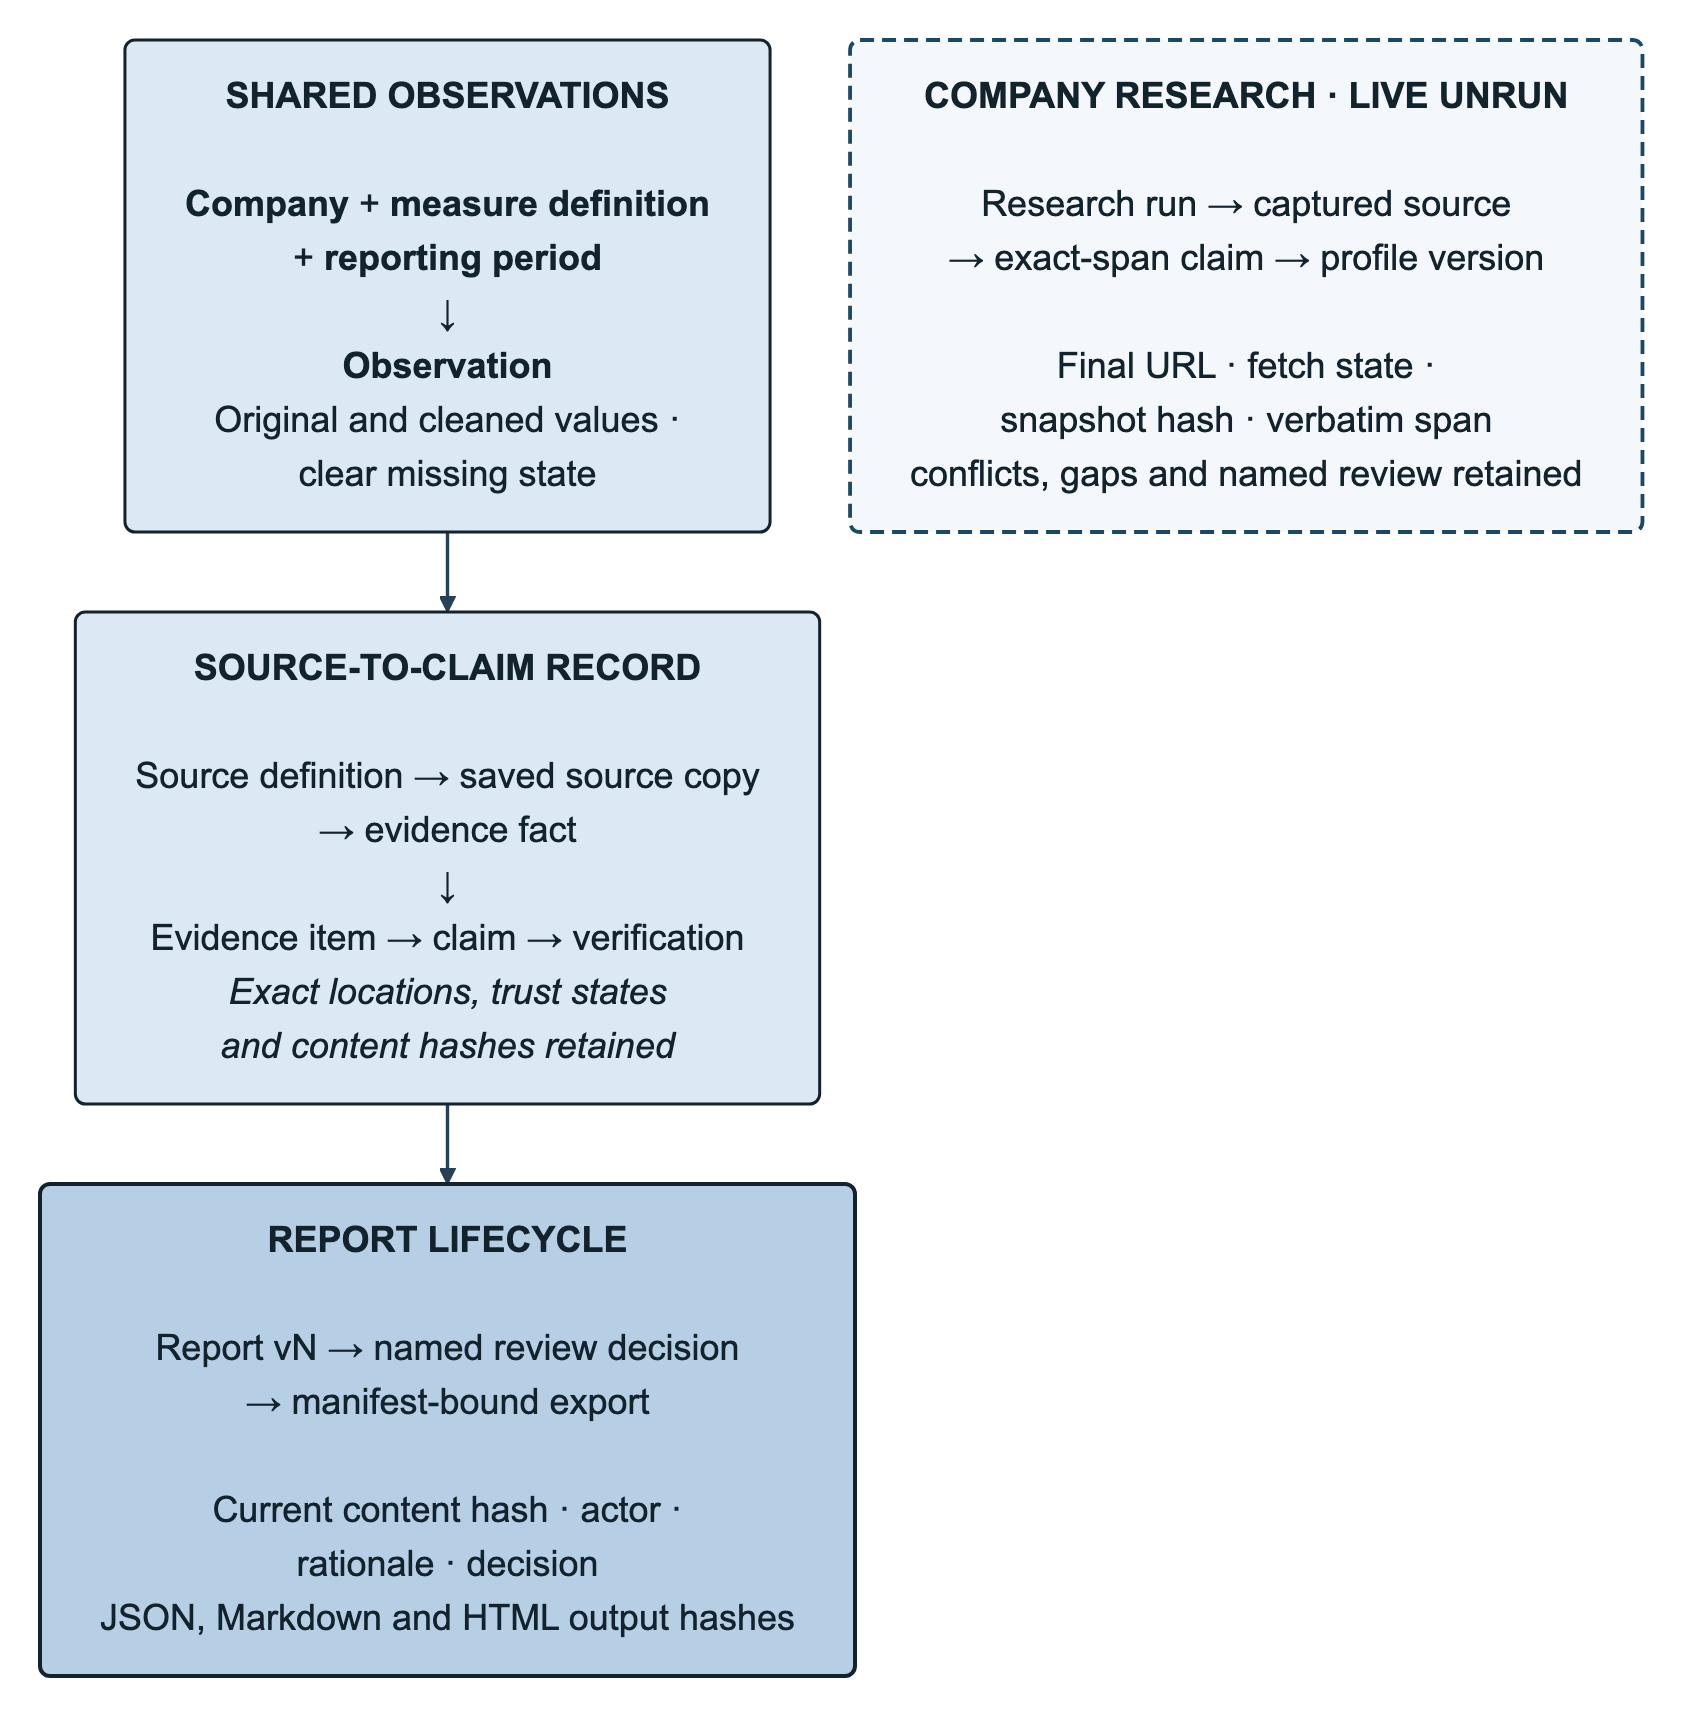
\includegraphics[width=\textwidth,height=0.82\textheight,keepaspectratio]{exhibits/sys_f2_canonical_data_provenance_model.png}
  \caption{Canonical data, provenance and approval lineage. Author synthesis of the implemented relational contracts. The dashed panel is the company-research track, which runs on its own records rather than as a stage of the portfolio chain.}
  \label{fig:sys-canonical-data-provenance-model}
\end{figure}
\clearpage
\section{Intake and legal-identity control}

The portfolio-import route accepts XLSX, CSV and JSON, then hashes the original bytes before writing a create-once snapshot. Its dataset identifier combines those bytes with the reporting-period label; a repeated hash and period reuses the stored submission only when classification, cutoff and profile remain compatible. Every company row then passes through the same identity resolver, and a conflicting identifier becomes a counted hold rather than a silent repair or merge \citep{pineau2021reproducibility,gebru2021datasheets}.

The company-intelligence route accepts a Companies House number without a name or website, tidying its format before checking its structure. A well-formed number creates an exact identifier, a placeholder company and a held case; crucially, it is not confirmed against the register, because valid shape is not proof of existence. Website, name-and-jurisdiction and document routes instead store what was submitted as a claim, leaving domains pending and document bytes untrusted and checksum-bound, since legal registration and operational identity are not the same thing \citep{galanakis2026chrt,hardman2023small}.

Identity becomes ready only after a named actor accepts the exact identifier with a substantive reason before source use. A rejection leaves identity unresolved; an identifier/name disagreement, a reused name with another number, a cross-classification collision, or a domain verified elsewhere is refused or held. Names may suggest a candidate, but neither name normalisation nor fuzzy similarity merges companies; name-only portfolio imports create unresolved records for review. This conservative choice sacrifices recall to reduce false joins, consistent with evidence that heterogeneous registers need cautious linkage and retain matching error \citep{thorne2026funding,surak2026gateways,galanakis2026chrt}.

A fingerprint over intake content, purpose, classification and contract versions means an exact repeat reuses the stored artefact rather than creating a duplicate, and source collection will not begin unless the reviewed number matches both the source key and the company. Figure~\ref{fig:sys-legal-identity-decision-flow} maps these gates, and direct live Companies House access remains held at gate G2 \citep{pineau2021reproducibility,galanakis2026chrt}.

\clearpage
\begin{figure}[p]
  \centering
  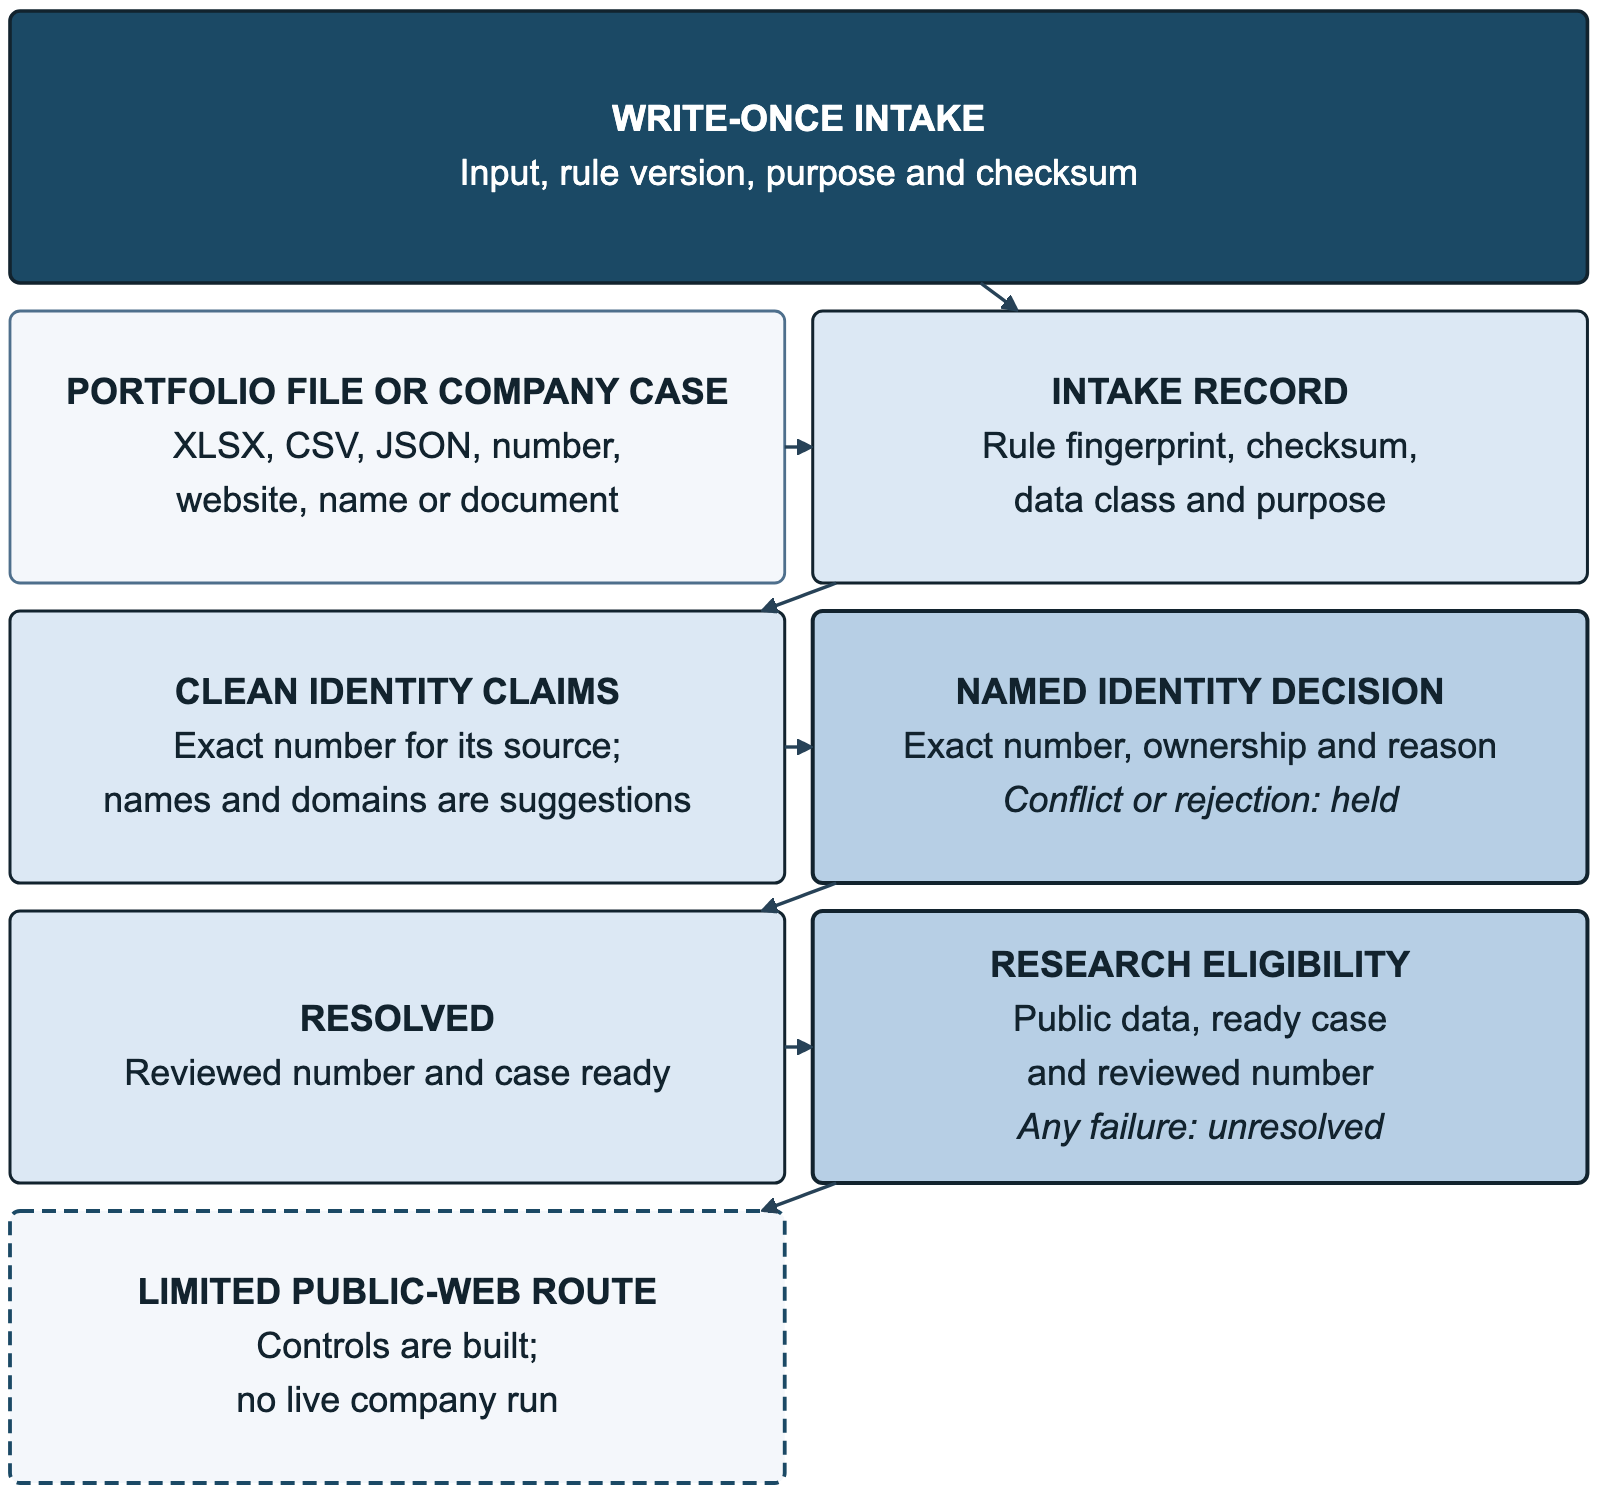
\includegraphics[width=\textwidth,height=0.82\textheight,keepaspectratio]{exhibits/sys_f3_legal_identity_decision_flow.png}
  \caption{Legal-identity intake, decision and downstream research gate. Author synthesis of the implemented local controls.}
  \label{fig:sys-legal-identity-decision-flow}
\end{figure}
\clearpage
\section{Fixed portfolio workflow and separate verification}

The implemented portfolio workflow follows eight fixed stages: plan, resolve identity, collect evidence, extract values, normalise them, verify claims, compose a report and stop at human review. Each stage has a named functional role and a persisted run record holding input and output hashes, status, timing and attempts. A failure is recorded and stops the stages that would have followed it, and unresolved identity stops collection before it starts. Because every stage leaves a record, a reader can later ask not only what the workflow produced but where it stopped and why \citep{pineau2021reproducibility,hevner2004design}.

Collection stores run-linked evidence and its time decision before extraction. Only temporally eligible, trusted public evidence reaches the extraction provider; untrusted material is counted and bypassed. A strict schema binds extracted company, metric, period, value and exact evidence locator, while deterministic metric rules then normalise type, unit, currency and missing state. Existing extractions are reused and every provider attempt is stored, including the failed ones \citep{gao2023alce,gao2023rarr,pineau2021reproducibility}.

Verification is the stage that decides what may be said. Before a claim is constructed, the workflow checks sourceability, provenance, period, trust, value and currency, then writes a verification record beside the claim. The verifier is a pure function returning one of five states: supported, contradicted, insufficient evidence, stale, or rejected as untrusted. A conflict between two current public sources cannot be averaged away into a compromise figure. Crucially, the verifier runs separately from the extractor and the composer and cannot rewrite their records, so a claim can be refused but not quietly repaired. This is separation of duties inside one program, not independent judgement by a second party \citep{gao2023alce,gao2023rarr,nist2023airmf}.

Composition places supported claims in the narrative and exposes other states as exceptions, then hashes the current, versioned report and moves it to pending review. A named reviewer may approve, reject or request an edit; each decision records actor, reason and report version. Editing creates a new section version, recalculates the content hash and revokes approval. Export remains unavailable until current approval, and optimistic locking plus a manifest-backed staged write guards stale or partial publication attempts \citep{amershi2019guidelines,bucinca2021forcing,pineau2021reproducibility}.

Two design choices are worth separating here, because they are often confused. The first is fixed orchestration over open-ended agent conversation: the workflow is a state machine with explicit stops, which removes uncontrolled branching and puts every failure in a locatable place, at the price of any adaptive planning. The second is role separation, which Section~\ref{sec:design-alternatives} argues for and this chapter implements. Its value lies in who may do what, not in how many components exist: the extractor cannot admit its own output, the verifier cannot rewrite what it judges, and neither can approve a report. Consistent with that section, a single program could apply the identical support rule, and the D0 comparison in Chapter~5 isolates that rule rather than the number of roles. Figure~\ref{fig:sys-fixed-workflow-verification-state-machine} maps these boundaries \citep{guo2024multiagent,wu2024autogen,peffers2007dsrm}.

\clearpage
\begin{figure}[p]
  \centering
  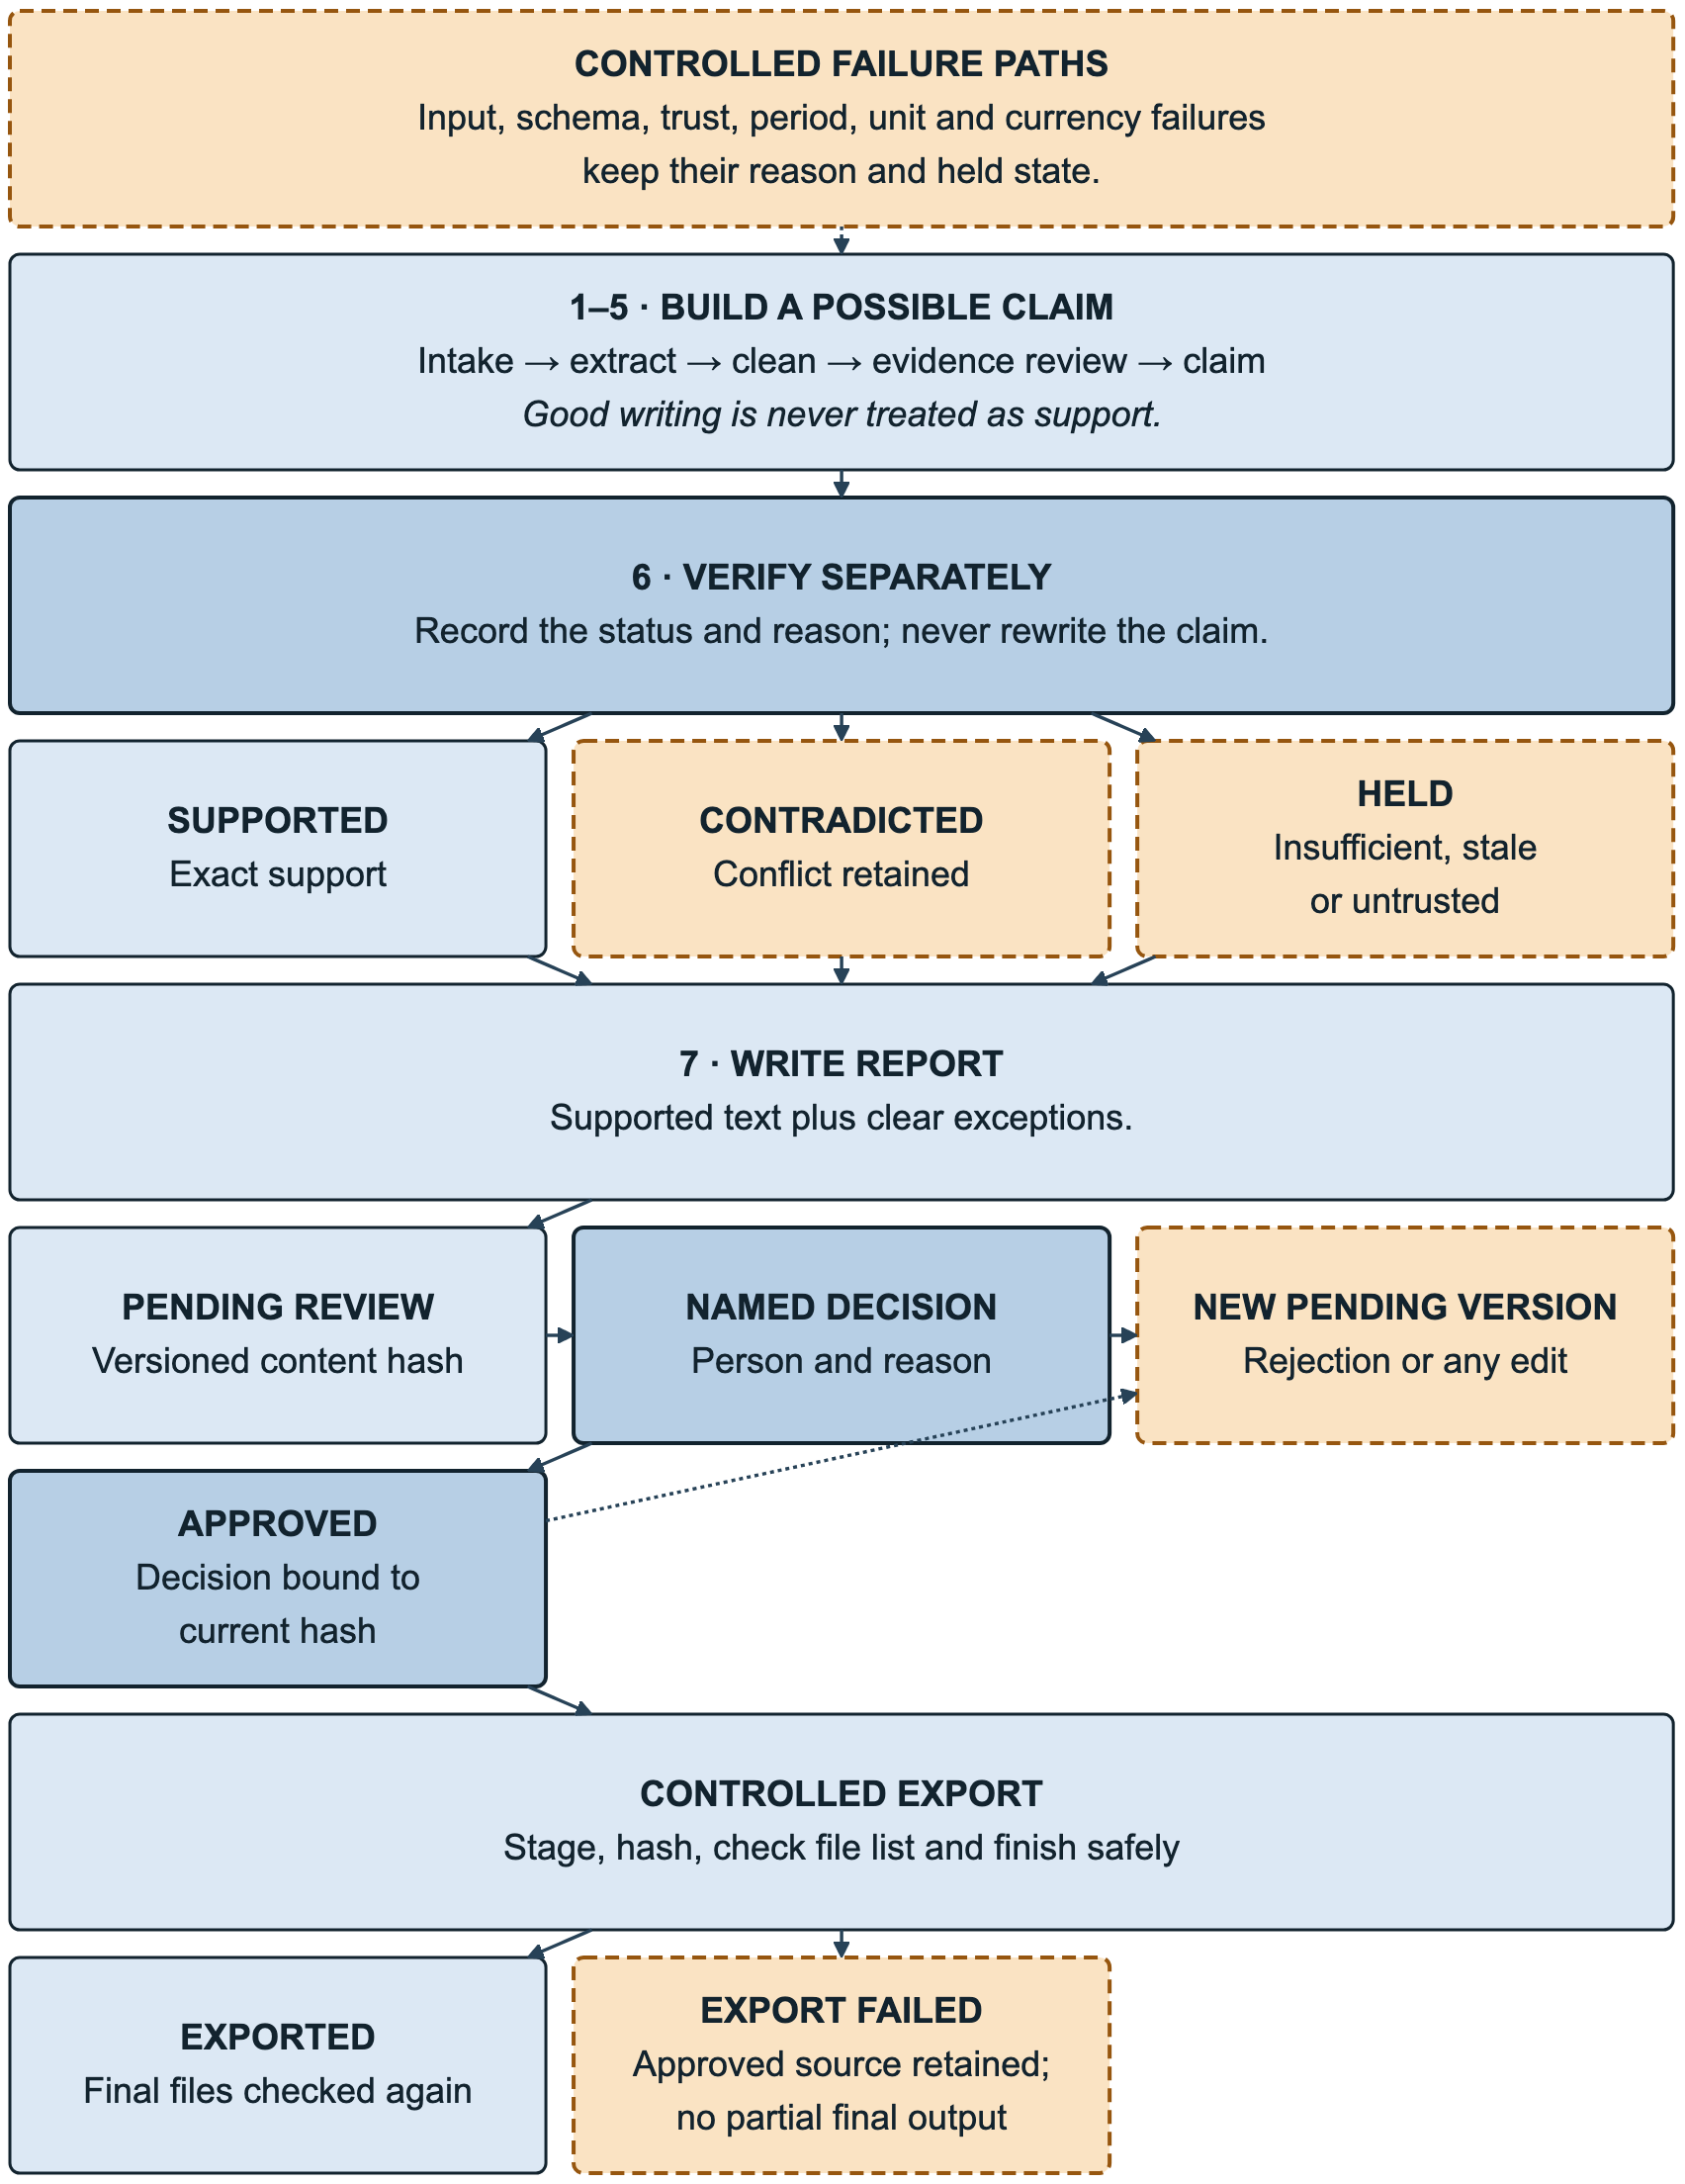
\includegraphics[width=\textwidth,height=0.82\textheight,keepaspectratio]{exhibits/sys_f4_fixed_workflow_verification_state_machine.png}
  \caption{Fixed workflow, separate verification states, named approval and controlled export. Author synthesis of the implemented local controls.}
  \label{fig:sys-fixed-workflow-verification-state-machine}
\end{figure}
\clearpage
\section{Fixed source connectors, time and quality}

The source layer is a registry of declared capabilities rather than a crawler. Every request names the source, company, reviewed identifier, cut-off, fact keys and mode, and the registry refuses it before any adapter runs if the capability is unsupported, the identity is unresolved, unreviewed or expired, or live retrieval is requested while admission is closed. A refusal of this kind is a decision not to look, which the system records differently from a publisher having no record \citep{gebru2021datasheets,pineau2021reproducibility}.

Two deterministic adapters are usable, both through synthetic offline replay. The Companies House adapter (manifest 1.4.0) matches an exact number and exposes company, filing and charge fields through JSON locators. The UKRI adapter (manifest 1.3.0) matches an exact organisation identifier, selects the most recent correction available at the cut-off, and emits stable project and outcome locators. Each replay stores the source version, the bytes, a checksum, the retrieval and publication times, and a derivation hash, so the same input can be re-examined later and shown to be the same input \citep{galanakis2026chrt,hardman2023small,pineau2021reproducibility}.

Time is judged relative to the claim, not to the moment of collection. Evidence is ineligible if it carries no recorded publication or availability time, was published after the reporting cut-off, takes effect in the future, or had expired before the period began; when it was retrieved is tracked separately. A cumulative figure must span exactly from the stored programme start to the cut-off. UKRI funding binds only when every award in the window carries a finite, explicit sterling amount, and otherwise leaves a missing state with a diagnostic rather than an inferred zero or an unauthorised currency conversion \citep{hardman2023small,kapoor2023leakage,nikiforova2020quality}.

The reasons a fact can be absent are then kept apart, because collapsing them would destroy the very distinction the report depends on. A lookup that finds nothing is \texttt{no\_record}; a source that could not be reached is \texttt{source\_unavailable}; a request refused before the adapter ran is a policy block; a value that fails validation is a typed missing state; and a collection problem that cannot be retried is \texttt{failed}. The quality contract built on these states excludes untrusted or time-ineligible evidence, holds incomplete provenance and conflicts, and warns on the bounded absence cases. Table~\ref{tab:sys-adapter-capability-state}, in Appendix~\ref{app:requirements-traceability}, maps the decisions, all of which remain bounded by the snapshots admitted, with live Companies House and UKRI retrieval held at gate G2 \citep{gao2023alce,gebru2021datasheets,nikiforova2020quality}.
\section{Bounded public-web company-research case study}

This section describes the one route that reaches outside the local machine, and the point of its
design is that search is allowed to suggest but never to supply. The path opens only after a public
case has a reviewed Companies House number and a fixed reporting cut-off. The Responses API then runs
\texttt{web\_search} with \texttt{store=False} to plan discovery, and the application admits only
canonical HTTPS addresses that also appear in the tool's own list of consulted sources. Page titles and
model prose stay metadata; they never become company facts \citep{openai2026websearch,gao2023alce}.

Application code, not the search result, then fetches each candidate. It refuses embedded credentials,
non-default ports, local hosts and addresses that do not resolve publicly; it checks robots rules,
re-validates every redirect, permits six textual content types, and enforces limits on elapsed time,
redirects and bytes. The connection is made to a verified public address while still checking the
hostname on the certificate. Every page that comes back is treated as hostile input, because hidden
instructions can travel inside remotely supplied content
\citep{greshake2023indirect,autio2024genai}.

What survives capture is converted to visible text, stripped of personal contact details, and stored
under a content hash in a directory that refuses to overwrite. Extraction sees only that bounded,
redacted text, and a proposed statement is admitted only if its address matches a captured source, the
statement equals the evidence passage, and that passage occurs literally in the stored text, with the
cut-off rule satisfied and any date or amount appearing inside the passage itself. A citation
therefore becomes something a reader can check rather than a mark implying that checking has happened
\citep{gao2023alce,gao2023rarr,autio2024genai}.

Four tasks run in order behind this -- discover, capture, extract and compose -- under one fingerprint
covering identity, cut-off, model, prompt, policy and budgets, so no task can start before its
prerequisite or resume under a changed contract, and every retry, token and byte is counted against
the run. Composition is then fixed rather than generative: it groups admitted claims, marks
multi-source disagreements for a named person, and lists the categories that were blocked,
unsupported, failed or simply not covered, so a gap stays visible instead of being smoothed out of a
persuasive narrative. Figure~\ref{fig:sys-company-research-funnel} summarises the funnel. Everything
described here ran against fake providers and controlled responses, which makes this route
implementation evidence that answers neither research question
\citep{nist2023airmf,gao2023alce,autio2024genai}.

\clearpage
\begin{figure}[p]
  \centering
  \caption{Bounded public-web evidence funnel}
  \label{fig:sys-company-research-funnel}
  \small
  \setlength{\tabcolsep}{6pt}
  \renewcommand{\arraystretch}{1.18}
  \begin{tabularx}{0.96\textwidth}{@{}P{0.15\textwidth}P{0.235\textwidth}Y P{0.20\textwidth}@{}}
    \toprule
    \textbf{Persisted stage} &
    \textbf{Input boundary} &
    \textbf{Deterministic admission gate} &
    \textbf{Persisted output / visible gap} \\
    \midrule

    \textbf{1 Discover} &
    Reviewed Companies House number, public case, cutoff and category plan. &
    Responses web search proposes URLs; accept only returned-source, canonical public HTTPS URLs.
    Search snippets and model statements have no evidential authority. &
    Bounded candidate inventory, source domains and model/tool usage. Missing categories remain
    uncovered. \\

    \addlinespace[3pt]
    \multicolumn{4}{c}{\Large$\downarrow$} \\
    \addlinespace[1pt]

    \textbf{2 Capture} &
    Candidate URL and pinned response, redirect, byte and elapsed budgets. &
    Robots, scheme, port, credentials, DNS, public-IP connection, hostname TLS, redirect, status,
    MIME and streaming-size checks. &
    Owner-scoped redacted snapshot, URL, time, MIME and hashes; blocked, unsupported or failed
    state with code. \\

    \addlinespace[3pt]
    \multicolumn{4}{c}{\Large$\downarrow$} \\
    \addlinespace[1pt]

    \textbf{3 Extract} &
    Bounded visible text with personal contacts redacted; all page text is untrusted data. &
    Exact captured URL; literal statement/span equality and containment; minimum span, cutoff,
    personal-data, recommendation and prompt-injection checks. &
    Admitted claim plus exact span and source locator, or explicit abstention. Returned model prose
    alone is discarded. \\

    \addlinespace[3pt]
    \multicolumn{4}{c}{\Large$\downarrow$} \\
    \addlinespace[1pt]

    \textbf{4 Compose} &
    Hash-ordered admitted claims and captured-source records. &
    Group by claim category and subject; retain attribution; flag multi-source disagreement; never
    infer recommendation or valuation. &
    Hash-bound pending-review profile with citations, contradictions, coverage counts, uncovered
    categories and limitations. \\
    \bottomrule
  \end{tabularx}

  \vspace{8pt}
  \fbox{\parbox{0.92\textwidth}{\centering\small
    \textbf{Cross-cutting control:} one serial persisted task at a time; bounded retries,
    cancellation, recovery, token/tool/model/byte/time telemetry and named approval before export.
    \textbf{Evidence state: IMPLEMENTED + SYNTHETICALLY TESTED; LIVE COMPANY RESEARCH UNRUN.}}}

  \vspace{6pt}
  \parbox{0.94\textwidth}{\scriptsize
    \textit{Source note:} Faye Niu's author synthesis of the current repository implementation and
    local synthetic tests. OpenAI (2026b, PDF pp.~1--3, 6) documents Responses web search and source
    URLs; Gao et al. (2023a, PDF pp.~1--3, 8--9) shows that citation quality and factual correctness
    require separate assessment; Greshake et al. (2023, PDF pp.~1--5, 25) and NIST (2024, PDF
    pp.~15--16, 44, 48) motivate treating retrieved content as untrusted and retaining risk controls,
    provenance and human review. These sources do not certify this implementation or establish live
    performance.}
\end{figure}
\clearpage

\section{Human review and controlled outputs}

The portfolio-report path stops at pending review. Approval or rejection requires the configured
reviewer identity, a substantive rationale and the current optimistic-lock token. Nobody can approve a
report until every claim in it carries a recorded verification, and any edit appends a new section
version, recalculates the report hash and cancels the previous decision. The effect is a deliberate
stopping point at which a named person, not the software, takes responsibility for release
\citep{amershi2019guidelines,bucinca2021forcing}.

Company-research profiles use a separate, narrower gate. Before a named approve or reject decision,
the service rechecks the profile hash, pinned run contract and completed composition task; stale
locks, altered content and unfinished recovery are refused. Contradiction candidates and coverage
gaps stay inside the dossier the reviewer sees, so a gap has to be looked at rather than discovered
later. Only approved profiles can be downloaded, as JSON or printable HTML
\citep{gao2023alce,nist2023airmf}.

For portfolio reports, export accepts only the current approved version and produces JSON, Markdown
and accessible HTML. Files are staged below the local export root, bound to a versioned manifest and
content hash, then re-verified before reuse, and a partial write is never marked as exported. Release
is therefore local and deliberate: the system writes files to a folder, it does not publish
\citep{pineau2021reproducibility,gebru2021datasheets,nist2023airmf}.
\section{Failure, recovery, and implementation-status ledger}

One principle runs through every control above: a failure keeps its own name and stays visible, so
that none of the distinct outcomes catalogued in Section~4.6 can quietly become a successful claim.
Retryable tasks keep their attempts and final reasons, and interrupted work resumes only under the
same run contract, so a retry is safe rather than hopeful
\citep{pineau2021reproducibility,nist2023airmf}.

Table~\ref{tab:sys-failure-recovery-status}, in Appendix~\ref{app:requirements-traceability}, then
separates tested engineering work from work that is on hold, and the distinction matters because a
reader can otherwise mistake a working feature for a tested outcome. The local workflow, source records, approval and export controls, offline connectors
and gated public-web route were built and tested with fictional or controlled inputs. Direct live
official-source access, a live public-web check, the fixed company comparison, authorised human
evaluation and production deployment were not run, exist only as plans, or fall outside scope
\citep{hevner2004design,peffers2007dsrm}.
